Una de las características más deseadas por parte de los usuarios de SIMDE 
(entre los que yo mismo me puedo incluir), es un sistema de errores más descriptivo. 

\bigskip
Por desgracia, en la versión original de SIMDE sólo se mostraba una notificación que indicaba
que el código cargado contenía errores.

\begin{figure}[!th]
\begin{center}
\includegraphics[width=0.5\textwidth]{images/cap6/errorsimde.eps}
\caption{Notificacion de error original SIMDE}
\end{center}
\end{figure}

Ahora, tras una serie de modificaciones en el parseador de código, se muestran los siguientes errores:

\begin{enumerate}
\item \textbf{Operando erróneo}.
\item \textbf{Opcode desconocido}.
\item \textbf{Etiqueta repetida}.
\end{enumerate}

Además, se muestra la línea del error. Esto resulta tremendamente importante, 
ya que una de los ejercicios que se propone en SIMDE requiere realizar mejoras en el rendimiento
de código haciendo uso de técnicas como el desenrollado de bucles, que dan lugar a códigos de considerable
longitud.

\begin{figure}[!th]
\begin{center}
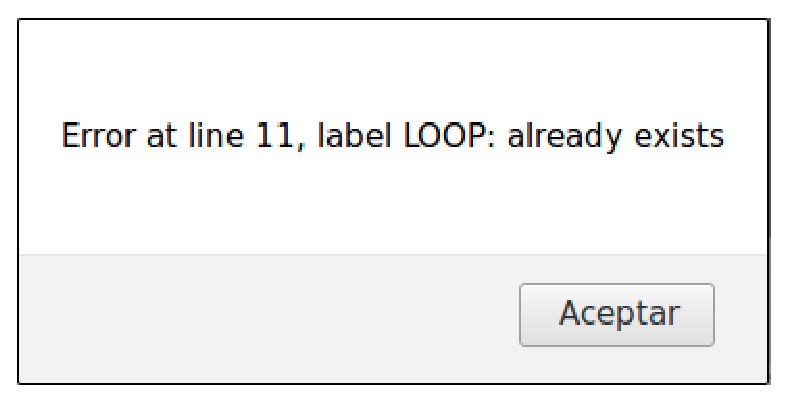
\includegraphics[width=0.5\textwidth]{images/cap6/nuevoerrorsimde.eps}
\caption{Ejemplos de errores en la nueva versión de simde}
\end{center}
\end{figure}
